\documentclass{article}

\usepackage[T1]{fontenc}
\usepackage{microtype}
\usepackage{graphicx}
\usepackage{booktabs}
\usepackage{amsmath}
\usepackage{amssymb}
\usepackage{hyperref}
\setlength{\emergencystretch}{2em}

\newcommand{\theHalgorithm}{\arabic{algorithm}}

\usepackage[accepted]{mlsys2025}

\makeatletter
\renewcommand{\mlsys@appearing}{Copyright 2026 by the author.}
\renewcommand{\Notice@String}{\mlsys@appearing}
\makeatother

\hypersetup{
  pdftitle={Versieve: Benchmarking Deterministic Document Extraction, Data Redaction, and Conformal Gatekeeping},
  pdfauthor={Gege Ardiyansyah},
  pdfsubject={Systems for Machine Learning}
}

\mlsystitlerunning{Versieve: Benchmarking Document Extraction and Data Redaction}

\begin{document}

\twocolumn[
\mlsystitle{Versieve: Benchmarking Deterministic Document Extraction, Data Redaction, and Conformal Gatekeeping}

\begin{mlsysauthorlist}
\textbf{Gege Ardiyansyah}
\end{mlsysauthorlist}

\mlsystitlerunning{Versieve: Benchmarking Document Extraction and Data Redaction}
\mlsyskeywords{WebAssembly, conformal prediction, Learn-Then-Test, PII de-identification, document curation, Graph-PPR, Cache-Augmented Generation}

\vskip 0.3in

\begin{abstract}
Preparing institutional documents for AI retrieval or post-training typically requires stripping boilerplate, redacting sensitive fields, and filtering low-quality passages. In clinical, legal, and regulated enterprise settings, raw records cannot be sent to cloud APIs for preprocessing, so the entire pipeline must run deterministically inside a local, auditable sandbox. We present \textbf{Versieve}, a zero-egress document curation, conformal gatekeeping, and local retrieval engine built around zero-import WebAssembly kernels and a single-header C99 core. We evaluate Versieve across a $1{,}207$-document public benchmark suite (ICDAR-2019 FUNSD, PubMedQA, PubMed Central full-text PDFs, and \texttt{ai4privacy-200k}) and a six-model open-weight compliance evaluation on an 8\,GB RTX~4070 Laptop GPU. Deterministic ingestion extracts readable prose from all $8/8$ PMC PDFs ($8{,}134$ lines, $55{,}099$ words in $209.02$\,ms) without raster OCR and preserves $97.38\%$ of FUNSD word boxes under $512{\times}512$ overlapping tiles. Format-validated regular expressions recall $78.6\%$ ($110/140$) of contact, card, and IPv4 spans, $49.6\%$ ($118/238$) of bare person names, and $31.0\%$ ($180/580$) across all $26$ structured PII tags, while a $334$-word exclusion lexicon reduces false-positive Title-Case hits on blind PubMedQA abstracts by $2.72\times$ ($5.46 \to 2.01$ per $1{,}000$ words). Above the regex layer, a 520-dimensional logistic gatekeeper calibrated via Learn-Then-Test (LTT) provides monotonic held-out risk control ($14.63\% \to 0.0\%$ conditional FPR) and fails closed cleanly at $\alpha=0.01$ when the unsafe calibration sample is below the theoretical floor ($n_{\text{cal,unsafe}}=206 < 299$, $\operatorname{BinomCDF}=0.1261 > 0.05$). Across runtime substrates, median process startup is $14.12$\,ms (C99) and $106.22$\,ms (Node+WASM) versus $12{,}917$\,ms for PyTorch+DuckDB. Finally, in downstream compliance QA across \texttt{Qwen2.5-0.5B-Instruct}, size-matched \texttt{Qwen2.5-1.5B-Instruct}, and \texttt{LFM3-1.7B-Base}, zero-training WebAssembly Graph-PPR retrieval (\texttt{verisieve\_graph.wasm}) significantly outperforms fair-shot assistant-only chat LoRA ($p = 0.001$ on blinded \texttt{qwen2.5:7b} judge; $p = 0.0005$ on token F1), while pre-processing PII redaction removes adversarial context extraction ($11/12 \to 0/12$) and lowers $20\times$-canary weight exposure by $4.93$--$5.70$ bits across all three models at zero QA accuracy loss.
\end{abstract}
]

\section{Introduction}
\label{sec:intro}

Domain-specific retrieval and post-training pipelines ingest heterogeneous institutional documents, including scientific PDFs, Word reports, web pages, and scanned forms \citep{soldaini2024dolma,penedo2024fineweb}. Standard curation stacks often rely on hosted language models or cloud de-identification services to remove boilerplate, detect personally identifiable information (PII), and filter noisy passages \citep{ai4privacy2023,presidio2021}. For clinical, legal, and confidential enterprise corpora, however, transmitting raw source documents to external endpoints violates organizational or regulatory data-residency boundaries.

Running curation locally introduces a distinct systems challenge. A practical client-side pipeline must be lightweight enough to start in milliseconds on standard laptops, deterministic enough to replay and audit every redaction decision, and statistically conservative enough to abstain rather than silently release sensitive records when a heuristic detector misses an unusual PII format.

We design and evaluate \textbf{Versieve}, a portable, zero-egress document preparation and retrieval stack organized across three explicit layers:
\begin{enumerate}
    \item \textbf{Interactive Web Workbench (RTIO):} A browser interface (\url{https://www.rtio.io/sandbox}) for inspecting documents, reviewing redactions and abstentions, labeling customer-specific chunks, and launching local open-weight workflows without uploading files.
    \item \textbf{Portable Curation and Gatekeeping Engine (Versieve):} A shared deterministic core implementing PDF and \texttt{.docx} parsing, multi-stage deduplication, salted-pseudonym PII redaction, 520-dimensional feature extraction, and finite-sample Learn-Then-Test (LTT) conformal gatekeeping across the browser, Node.js CLI, Model Context Protocol (MCP) server, and a $2{,}129$\,B single-header C99 library (\texttt{include/verisieve.h}).
    \item \textbf{Zero-Import WebAssembly Kernels:} Four standalone WASM binaries audited to have zero host imports: \texttt{verisieve\_clean.wasm} ($14{,}633$\,B) for text normalization, deduplication, and token-window chunking; \texttt{verisieve\_graph.wasm} ($54{,}402$\,B) for Dual-CSR document knowledge graphs, personalized PageRank (PPR), GDPR Art.~17 blast-radius eviction, shortest paths, Tarjan SCC, and Louvain clustering; \texttt{verisieve\_dl.wasm} ($60{,}096$\,B, $26$ \texttt{mle\_dl\_*} exports) for BitNet encoding, VeRA adapter training, and 64-dimensional needle retrieval \citep{wang2024bitnet,kopiczko2024vera,vaswani2017attention}; and \texttt{verisieve\_sql.wasm} ($49{,}642$\,B) for local SQL filtering. Optical character recognition (OCR) is isolated in a separate \texttt{cactus.wasm} module ($1{,}240{,}671$\,B) that fails closed whenever local OCR weights are absent.
\end{enumerate}

\begin{table}[t]
\caption{Summary of Versieve capabilities, verified measurements, and explicit operating boundaries.}
\label{tab:scope}
\vskip 0.08in
\begin{center}
\resizebox{\columnwidth}{!}{%
\begin{tabular}{lp{1.55in}p{1.35in}}
\toprule
\textbf{Subsystem} & \textbf{Verified Behavior} & \textbf{Operating Boundary} \\
\midrule
Web/Link Capture & Strips $53.7\%$ HTML boilerplate in $1.345$\,ms; blocks private IPs & Live remote fetch requires outbound network \\
PDF \& Word Files & Extracts \texttt{.docx} in $2.477$\,ms; $8/8$ PMC PDFs in $209.02$\,ms & Image-only PDFs require local OCR weights \\
Dedupe \& Manifest & SHA-256 + 3-gram Jaccard ($\ge 0.85$); signed provenance hash & Per-shard in-memory ring, not TB streaming \\
Conformal Gate & \texttt{safe} certifies at $\tau=0.55$; fails closed when $n_{\text{cal}}$ is too small & Small calibration sets yield conservative abstention \\
Local Substrates & C99 spawn $14.12$\,ms; NumPy wins shared logistic ($0.207$\,ms) & Warm compute varies by kernel architecture \\
\bottomrule
\end{tabular}%
}
\end{center}
\vskip -0.14in
\end{table}

Table~\ref{tab:scope} summarizes each subsystem alongside its explicit operating boundary, and Figure~\ref{fig:redaction-arch} traces the end-to-end flow of raw documents through ingestion, zero-import cleaning, salted-pseudonym redaction, and fail-closed conformal routing. The rest of this paper evaluates deterministic document ingestion (Section~\ref{sec:ingestion}), the public benchmark suite and testbed (Section~\ref{sec:datasets}), deterministic PII disambiguation and its recall ceiling (Section~\ref{sec:pii}), fail-closed LTT conformal gatekeeping (Section~\ref{sec:ltt}), runtime substrate trade-offs and downstream open-weight LLM adaptation (Section~\ref{sec:substrates}), and limitations (Section~\ref{sec:limitations}).

\begin{figure*}[t]
\centering
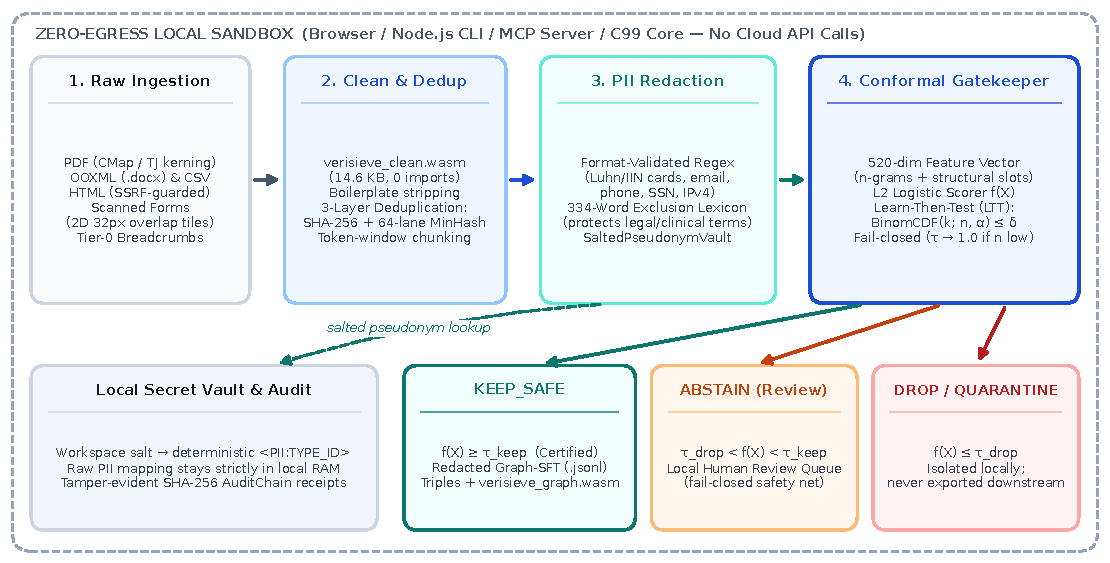
\includegraphics[width=0.98\textwidth]{figs/fig0-redaction-architecture.pdf}
\caption{End-to-end zero-egress Versieve extraction, redaction, and conformal gatekeeping architecture. Raw documents enter the local sandbox, pass through deterministic parsing and zero-import WebAssembly deduplication (\texttt{verisieve\_clean.wasm}), undergo format-validated PII redaction backed by a local-only \texttt{SaltedPseudonymVault} and a $334$-word exclusion lexicon, and are routed by the fail-closed Learn-Then-Test (LTT) gatekeeper into certified exports (\texttt{KEEP\_SAFE}), human review (\texttt{ABSTAIN}), or local quarantine (\texttt{DROP}).}
\label{fig:redaction-arch}
\end{figure*}

\section{Deterministic Document Ingestion and Layout Preservation}
\label{sec:ingestion}

Reliable downstream filtering and retrieval depend on converting raw binary and markup formats into clean, provenance-tracked text blocks without silently dropping content.

\subsection{HTML Stripping, OOXML Parsing, and Deduplication}
On the portable ingestion micro-benchmark, Versieve strips raw HTML boilerplate by $53.7\%$ ($503$\,B raw HTML to $233$\,B clean prose) in $1.345$\,ms, extracts $150$ characters from a $295$\,B native \texttt{.docx} OOXML container (including bit-3 ZIP data-descriptor archives) in $2.477$\,ms, and executes two-stage deduplication (exact SHA-256 plus 3-gram Jaccard similarity at $\ge 0.85$) across $5$ inputs into $4$ unique chunks in $0.554$\,ms. Emitting a signed manifest over $2$ sources and $50$ tokens (SHA-256 prefix \texttt{2de7618c79d41782}) completes the combined four-stage micro-benchmark in $5.393$\,ms.

\subsection{Native PDF CMap and Kerning Reconstruction}
Many scientific and regulatory PDFs embed custom glyph encodings rather than plain ASCII strings. Versieve's native parser (\texttt{extractPdfDiagnostics}) scans each PDF content stream in a single pass, resolves scoped 1-byte and 2-byte \texttt{/ToUnicode} CMap tables (\texttt{beginbfchar} and \texttt{beginbfrange}), and inserts word spaces whenever a PDF \texttt{TJ} operator specifies a negative kerning displacement of $\le -110$ glyph units.

Across all $8$ open-access PubMed Central (PMC) clinical PDFs in our evaluation suite, $7$ contain embedded \texttt{/ToUnicode} CMap streams and $2$ contain hex-encoded strings ($1$ and $57$ hex-decoded lines). Versieve recovers readable prose from all $8/8$ documents---$8{,}134$ lines and $55{,}099$ words---in $209.02$\,ms total ($26.13$\,ms per paper; range $8.42$\,ms to $64.54$\,ms) without invoking raster OCR.

\subsection{2D Overlapping Tiling for Scanned Forms}
When documents exist only as page images, naive downscaling destroys small form fields before an OCR model can read them. On all $199$ scanned forms in the ICDAR-2019 FUNSD dataset \citep{jaume2019funsd} ($30{,}595$ annotated word boxes), we evaluate how many word boxes remain geometrically legible ($\ge 8$\,px height and $\ge 4$\,px width after scaling) under five rasterization strategies (Table~\ref{tab:funsd}).

\begin{table}[t]
\caption{Geometric word-box survival on $199$ ICDAR-2019 FUNSD forms ($30{,}595$ boxes; legibility threshold $\ge 8{\times}4$\,px).}
\label{tab:funsd}
\vskip 0.08in
\begin{center}
\resizebox{\columnwidth}{!}{%
\begin{tabular}{lrrl}
\toprule
\textbf{Rasterization Strategy} & \textbf{Survived} & \textbf{Rate} & \textbf{Primary Failure Mode} \\
\midrule
Capped at 8 Reads & $1{,}592$ & $5.20\%$ & Read budget drops dense fields \\
Untiled $512{\times}512$ Scale & $6{,}281$ & $20.53\%$ & Small labels shrink below $8{\times}4$\,px \\
Horizontal 1D Bands ($512$\,px) & $21{,}811$ & $71.29\%$ & Aspect compression and seam cuts \\
2D Grid (Zero Overlap) & $28{,}283$ & $92.44\%$ & $4.94\%$ lost on tile boundaries \\
\textbf{2D Grid ($32$\,px Overlap)} & $\mathbf{29{,}793}$ & $\mathbf{97.38\%}$ & Avg.\ $6$ tiles/form ($6.29$\,ms scan) \\
\bottomrule
\end{tabular}%
}
\end{center}
\vskip -0.14in
\end{table}

Untiled $512{\times}512$ downscaling preserves only $20.53\%$ of word boxes, while a non-overlapping 2D grid still severs $4.94\%$ of words along tile seams. Adding a $32$\,px overlap across a $512{\times}512$ 2D grid raises geometric survival to $97.38\%$ ($29{,}793 / 30{,}595$ boxes) at an average of $6$ tiles per form and $6.29$\,ms total geometry computation.

\section{Evaluation Corpus and Hardware Testbed}
\label{sec:datasets}

Core curation, PII disambiguation, conformal calibration, and substrate benchmarks run over a unified $1{,}207$-document public corpus combining real archival and biomedical documents with span-annotated synthetic PII records (Table~\ref{tab:datasets}). Under the format-validated scanner, $826$ documents are labeled unsafe and $381$ safe ($68.43\%$ unsafe prevalence).

\begin{table}[t]
\caption{Public benchmark corpus ($1{,}207$ documents; $826$ unsafe, $381$ safe under format-validated labeling).}
\label{tab:datasets}
\vskip 0.08in
\begin{center}
\resizebox{\columnwidth}{!}{%
\begin{tabular}{llll}
\toprule
\textbf{Dataset} & \textbf{Provenance} & \textbf{Docs} & \textbf{Evaluation Role} \\
\midrule
ICDAR FUNSD \citep{jaume2019funsd} & Real scanned forms & $199$ & $30{,}595$ word boxes; tiling geometry \\
\texttt{ai4privacy-200k} \citep{ai4privacy2023} & Synthetic English & $500$ & $56$-tag PII span recall benchmark \\
PubMedQA \citep{jin2019pubmedqa} & Real clinical abstracts & $500$ & $250/250$ lexicon split; Needle QA \\
PMC full text \citep{miu_2017_pmc5773420} & Real clinical PDFs & $8$ & $8{,}134$ lines / $55{,}099$ words \\
\midrule
\textbf{Combined Suite} & \textbf{Real + Synthetic} & $\mathbf{1{,}207}$ & \textbf{$826$ unsafe / $381$ safe ($68.43\%$)} \\
\bottomrule
\end{tabular}%
}
\end{center}
\vskip -0.14in
\end{table}

\paragraph{Hardware and Software Environment.}
All benchmarks and GPU ablations ran locally on a single laptop: AMD Ryzen~7 7840HS ($8$ cores / $16$ threads), $31.3$\,GB RAM, NVIDIA GeForce RTX~4070 Laptop GPU ($8$\,GB VRAM), Windows~11 Home, Node.js v24.13.1, GCC~14.2.0 (MSYS2, C99 \texttt{-O3} binary $135{,}025$\,B), Python~3.12.4, NumPy~2.4.3, DuckDB~1.5.5, PyTorch~2.10.0+cpu (CPU substrate trials), and PyTorch~2.10.0+cu128 (local GPU LoRA training and inference).

\section{PII Disambiguation and the Deterministic Regex Ceiling}
\label{sec:pii}

\begin{figure*}[t]
\centering
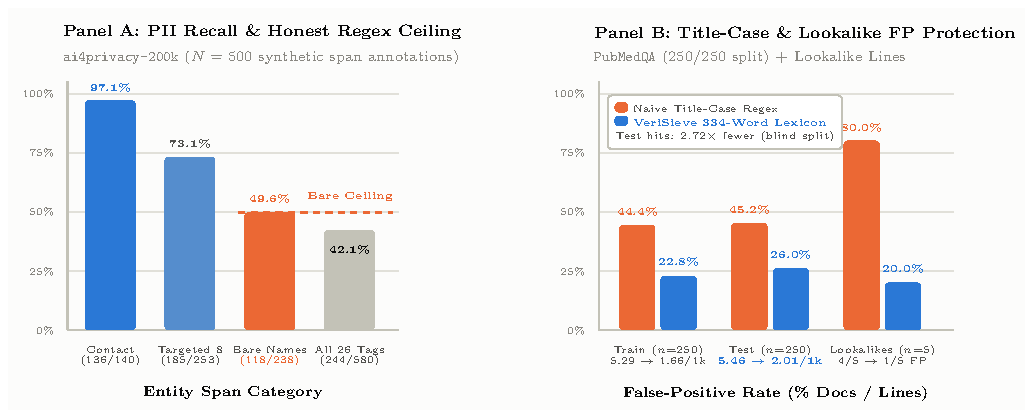
\includegraphics[width=0.96\textwidth]{figs/fig2-pii-disambiguation.pdf}
\caption{Format-validated PII scanning recall and false-positive reduction. \textbf{Panel A:} On $500$ \texttt{ai4privacy-200k} records, recall reaches $78.6\%$ ($110/140$) on contact, card, and IPv4 spans, $62.8\%$ ($159/253$) on the eight targeted patterns, $49.6\%$ ($118/238$) on bare person names, and $31.0\%$ ($180/580$) across all $26$ structured tags. \textbf{Panel B:} On the blind $250$-abstract PubMedQA split, the $334$-word exclusion lexicon cuts false-positive Title-Case matches by $2.72\times$ ($5.46 \to 2.01$ hits per $1{,}000$ words).}
\label{fig:pii}
\end{figure*}

Regular-expression PII scrubbers face a sharp precision--recall trade-off on scientific and legal documents. Aggressive Title-Case rules corrupt domain terminology (such as anatomical names, statistical methods, or statutory headings), whereas overly narrow patterns miss unprefixed human names and loosely formatted identifiers.

Versieve addresses precision in two ways. First, credit-card and financial identifier rules enforce Luhn checksum and Issuer Identification Number (IIN) validation so that arbitrary 16-digit scientific constants or grant IDs are not masked. Second, a pre-committed $334$-word exclusion lexicon (\texttt{EXCLUDED\_NAME\_WORDS}) suppresses common capitalized non-person phrases. On the held-out blind half of PubMedQA ($250$ clinical abstracts, $63{,}739$ words), the exclusion lexicon cuts false-positive Title-Case matches from $348$ ($5.46$ per $1{,}000$ words; $45.2\%$ of documents) down to $128$ ($2.01$ per $1{,}000$ words; $26.0\%$ of documents)---a $2.72\times$ reduction (Figure~\ref{fig:pii}, Panel~B). On the development half ($62{,}620$ words), hits similarly decline from $5.29$ to $1.66$ per $1{,}000$ words ($44.4\% \to 22.8\%$ of documents), and false alarms on a five-item technical lookalike suite drop from $4/5$ to $1/5$.

At the same time, evaluating the validated scanner against ground-truth spans on $500$ \texttt{ai4privacy-200k} records exposes a clear recall ceiling (Figure~\ref{fig:pii}, Panel~A): recall is $78.6\%$ ($110/140$) on contact, card, and IPv4 spans, $62.8\%$ ($159/253$) across the eight targeted identifier patterns, $49.6\%$ ($118/238$) on bare unprefixed person names, and $31.0\%$ ($180/580$) across all $26$ structured privacy tags (which include free-form addresses, employers, and usernames). Because deterministic regex alone cannot guarantee zero leakage on unstructured prose, Versieve treats regex as a fast first-pass redactor and places a statistically calibrated gatekeeper above it.

\section{Fail-Closed Conformal Gatekeeping}
\label{sec:ltt}

\begin{figure*}[t]
\centering
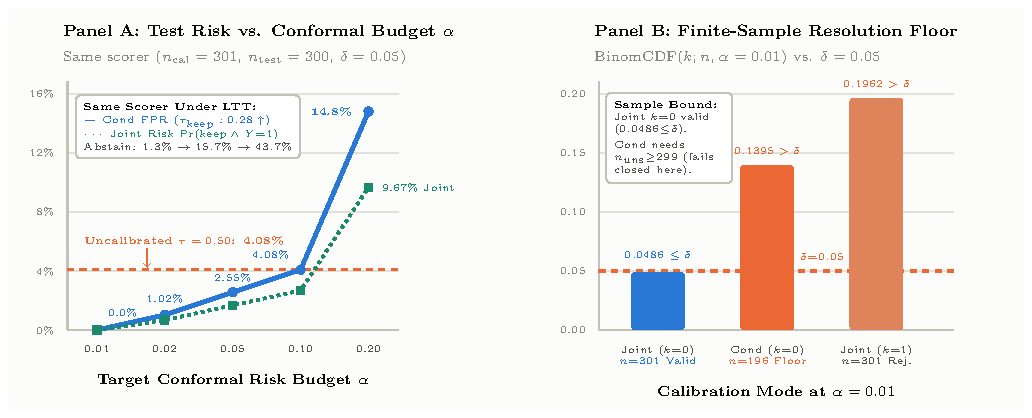
\includegraphics[width=0.96\textwidth]{figs/fig1-ltt-calibration.pdf}
\caption{Learn-Then-Test (LTT) calibration of the 520-dimensional L2 logistic gatekeeper ($n_{\text{train}}=607$ with $415$ unsafe; $n_{\text{cal}}=301$ with $206$ unsafe; $n_{\text{test}}=299$ with $205$ unsafe and $94$ safe; $\delta=0.05$). \textbf{Panel A:} Held-out conditional FPR and joint risk decrease monotonically as $\alpha$ tightens from $0.20$ to $0.01$, while abstention rises from $0.33\%$ to $40.8\%$. The dashed marker shows the uncalibrated $\tau=0.50$ baseline ($4.39\%$ conditional FPR). \textbf{Panel B:} At $\alpha=0.01$, joint risk over $n_{\text{cal}}=301$ certifies at $k=0$ ($\operatorname{BinomCDF}=0.0486 \le 0.05$), whereas conditional risk over $n_{\text{cal,unsafe}}=206 < 299$ yields $\operatorname{BinomCDF}=0.1261 > 0.05$ and fails closed.}
\label{fig:ltt}
\end{figure*}

Each document chunk is mapped to a 520-dimensional feature vector combining hashed lexical $n$-grams with structural metadata (scanner hit counts, token ratios, and extraction confidence) and scored by an L2-regularized logistic model $f(X) \in [0, 1]$ executed identically in JavaScript and float32 C99.

\subsection{Three-Way Decision Rule and Binomial Risk Control}
Given an upper acceptance threshold $\tau_{\text{keep}}$ and a drop floor $\tau_{\text{drop}} = \min(0.25, \tau_{\text{keep}})$, Versieve routes every chunk to one of three deterministic actions:
\begin{equation}
\resizebox{0.98\columnwidth}{!}{$\displaystyle
\operatorname{Action}(X) =
\begin{cases}
\texttt{KEEP\_SAFE}, & f(X) \ge \tau_{\text{keep}}, \\
\texttt{DROP\_OR\_QUARANTINE}, & f(X) \le \tau_{\text{drop}}, \\
\texttt{ABSTAIN\_HUMAN\_REVIEW}, & \tau_{\text{drop}} < f(X) < \tau_{\text{keep}}.
\end{cases}$}
\end{equation}

To select $\tau_{\text{keep}}$ with a finite-sample risk guarantee, we apply Learn-Then-Test \citep{angelopoulos2021ltt}. A candidate threshold is certified at target error budget $\alpha$ and confidence level $1-\delta$ ($\delta=0.05$) if and only if
\begin{equation}
\operatorname{BinomCDF}(k; n, \alpha) = \sum_{j=0}^{k} \binom{n}{j} \alpha^j (1-\alpha)^{n-j} \le \delta,
\end{equation}
where $k$ counts the unsafe calibration chunks accepted above $\tau$. Controlling \emph{conditional} false-positive risk sets $n = n_{\text{cal,unsafe}}$; controlling \emph{joint} false-accept risk sets $n = n_{\text{cal}}$. Critically, if no threshold satisfies the binomial inequality for the available calibration sample size, the calibrator fails closed by setting $\tau_{\text{keep}} = 1.0$, refusing to issue an unsupported certificate.

\subsection{Single-Scorer Risk--Yield Trade-Off}
We partition the $1{,}207$-document suite into stratified splits of $n_{\text{train}}=607$ ($415$ unsafe), $n_{\text{cal}}=301$ ($206$ unsafe), and $n_{\text{test}}=299$ ($205$ unsafe, $94$ safe), preserving $68.37\%$--$68.56\%$ unsafe prevalence across splits. Sweeping a single trained scorer over $\alpha \in [0.01, 0.20]$ demonstrates smooth, monotonic control of conditional FPR, joint risk, safe yield, and human-review abstention (Table~\ref{tab:ltt} and Figure~\ref{fig:ltt}).

\begin{table}[t]
\caption{Single-scorer LTT sweep ($n_{\text{cal}}=301$, $n_{\text{test}}=299$, $\delta=0.05$; $\tau_{\text{drop}}=0.25$ whenever $\tau_{\text{keep}} \ge 0.25$).}
\label{tab:ltt}
\vskip 0.08in
\begin{center}
\resizebox{\columnwidth}{!}{%
\begin{tabular}{lrrrrrl}
\toprule
\textbf{Setting} & $\boldsymbol{\tau_{\text{keep}}}$ & \textbf{Cond.\ FPR} & \textbf{Joint Risk} & \textbf{Safe Yield} & \textbf{Abstain} & \textbf{Certificate ($\delta=0.05$)} \\
\midrule
$\alpha = 0.20$ & $0.26$ & $14.63\%$ & $10.03\%$ & $96.81\%$ & $0.33\%$ & Certified (cond \& joint) \\
Uncalibrated & $0.50$ & $4.39\%$ & $3.01\%$ & $90.43\%$ & $0.00\%$ & Uncertified baseline \\
$\alpha = 0.10$ & $0.44$ & $4.88\%$ & $3.34\%$ & $92.55\%$ & $8.36\%$ & Certified (cond \& joint) \\
$\alpha = 0.05$ & $0.52$ & $3.41\%$ & $2.34\%$ & $89.36\%$ & $10.37\%$ & Certified (cond \& joint) \\
$\alpha = 0.02$ & $0.60$ & $0.98\%$ & $0.67\%$ & $82.98\%$ & $14.05\%$ & Certified (cond \& joint) \\
$\alpha = 0.01$ & $1.00$ & $0.00\%$ & $0.00\%$ & $0.00\%$ & $40.8\%$ & Joint valid / cond fail-closed \\
\bottomrule
\end{tabular}%
}
\end{center}
\vskip -0.14in
\end{table}

At $\alpha=0.01$ and $\delta=0.05$, certifying conditional risk with zero violations ($k=0$) requires at least $\lceil \ln(0.05)/\ln(0.99) \rceil = 299$ unsafe calibration items. Because our calibration split holds $n_{\text{cal,unsafe}}=206 < 299$, $\operatorname{BinomCDF}(0; 206, 0.01) = 0.1261 > 0.05$, so conditional calibration properly fails closed ($\tau_{\text{keep}}=1.0$, $40.80\%$ abstention), whereas joint risk over $n_{\text{cal}}=301$ certifies at $k=0$ ($\operatorname{BinomCDF}=0.0486 \le 0.05$).

On $124$ within-domain PubMedQA test items with injected contact tokens, syntax-driven contact regex achieves $100.0\%$ accuracy, the 520-dim logistic achieves $87.9\%$, and a naive any-PII Title-Case regex drops to $52.4\%$. Thus, regex excels on rigidly formatted identifiers, while the learned gate extends control to customer-defined quality and topicality criteria that cannot be expressed as regular expressions.

\subsection{Customer 100-Label Multi-Axis Gate}
Enterprise curation frequently demands a conjunction of three criteria: \texttt{safe} (privacy-clean), \texttt{useful} (substantive prose rather than navigation scraps), and \texttt{topic} (in-domain relevance). To test low-label cold starts, we train three independent logistic heads on $60$ customer-labeled chunks, calibrate on $40$ held-out labels, and evaluate on $300$ unseen documents (Table~\ref{tab:multiaxis}).

\begin{table}[t]
\caption{Customer 100-label multi-axis gate ($60$ train, $40$ calibration, $300$ held-out). Uncertifiable heads fail closed at $\tau_{\text{keep}}=1.0$.}
\label{tab:multiaxis}
\vskip 0.08in
\begin{center}
\resizebox{\columnwidth}{!}{%
\begin{tabular}{lrrrrl}
\toprule
\textbf{Gate Axis} & $\boldsymbol{\tau_{\text{keep}} / \tau_{\text{drop}}}$ & \textbf{Recall} & \textbf{Precision} & \textbf{Abstain} & \textbf{Calibration Outcome} \\
\midrule
\texttt{safe} & $0.55 / 0.33$ & $97.1\%$ & $95.7\%$ & $7.3\%$ & Certified safety head \\
\texttt{useful} & $1.00 / 0.05$ & --- & --- & $79.7\%$ & Fail-closed (insufficient cal) \\
\texttt{topic} & $1.00 / 0.25$ & --- & --- & $40.0\%$ & Fail-closed (insufficient cal) \\
\midrule
\textbf{Conjunction} & Combined & $0\%$ kept & --- & $28.3\%$ & \textbf{$0$ kept / $85$ abstain / $215$ drop} \\
\bottomrule
\end{tabular}%
}
\end{center}
\vskip -0.14in
\end{table}

The \texttt{safe} head certifies cleanly ($\tau_{\text{keep}}=0.55$, $\tau_{\text{drop}}=0.33$), achieving $97.1\%$ recall and $95.7\%$ precision at $7.3\%$ abstention. By contrast, with only $40$ total calibration chunks, the \texttt{useful} and \texttt{topic} heads lack enough negative calibration examples to clear the binomial test and both fail closed ($\tau_{\text{keep}}=1.0$). Consequently, the three-way conjunction conservatively releases $0$ chunks, routes $85$ ($28.3\%$) to human review, and drops $215$. Rather than masking insufficient calibration data behind an unverified threshold, fail-closed LTT forces the operator to supply additional labeled calibration rows before automated release begins.

\paragraph{Hierarchical Cluster-Robust Conformal Risk Control (\texttt{HC-CRC}) and Streaming Martingales (\texttt{E-LTT}).}
When calibration units are multi-paragraph documents $D_m = \{c_{m,1},\dots,c_{m,N_m}\}$ rather than independent abstracts, chunks within the same document exhibit intra-cluster correlation $\rho > 0$, inflating variance by the Cluster Design Effect $\operatorname{DEFF} = 1 + (\bar{N}_u - 1)\rho$. Versieve extends the gatekeeper (\texttt{calibrateClusterRobustGatekeeper} and \texttt{calibrateStreamingEProcessGatekeeper} in \texttt{src/gatekeeper.js}) to define the bounded cluster loss $L_m(\lambda) = |U_m|^{-1} \sum_{c \in U_m} \mathbb{I}[f(c) \ge \lambda] \in [0, 1]$ over the unsafe blocks $U_m \subseteq D_m$ of exchangeable parent documents $m=1,\dots,M_0$, inverting the $\operatorname{DEFF}$-adjusted effective sample size $N_{\text{eff}} = \lfloor n_0 / \operatorname{DEFF} \rfloor$ (\texttt{HC-CRC}) or maintaining the anytime-valid Ville betting supermartingale $\mathcal{E}_t(\lambda) = \prod_{m=1}^t (1 + \gamma_m(\alpha - L_m(\lambda))) \ge 1/\delta$ (\texttt{E-LTT}) for streaming ingestion.

\section{Runtime Substrates, Local Retrieval, and Open-Weight Adaptation}
\label{sec:substrates}

\begin{figure*}[t]
\centering
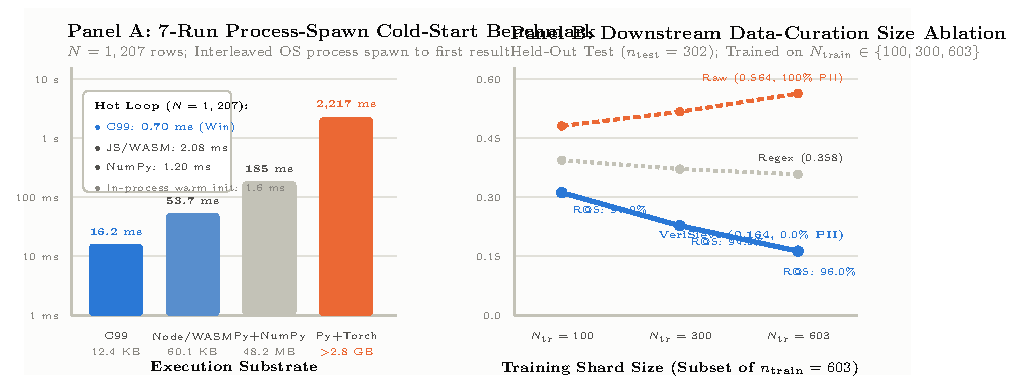
\includegraphics[width=0.96\textwidth]{figs/fig3-substrate-and-scaling.pdf}
\caption{Runtime substrate overhead and held-out learning curves. \textbf{Panel A:} Median OS process startup across $7$ interleaved runs: C99 ($14.12$\,ms), Node+WASM ($106.22$\,ms, $121.6\times$ faster than PyTorch+DuckDB at $12{,}917$\,ms), and Python+NumPy ($388.79$\,ms). Peak RSS is $6.08$, $55.97$, $31.49$, and $432.3$\,MB, respectively. \textbf{Panel B:} Held-out loss ($n_{\text{test}}=299$) as $N_{\text{train}}$ increases from $100$ to $607$: Gate BCE falls $0.2577 \to 0.189$ and WASM VeRA BCE falls $0.9432 \to 0.6141$, while Needle R@5 remains steady at $60.0\%$.}
\label{fig:substrates}
\end{figure*}

\subsection{Process Startup vs.\ Warm Kernel Compute}
Interactive CLI tools, browser extensions, and MCP servers spawn short-lived processes frequently, making cold startup latency and memory footprint first-order design constraints. Table~\ref{tab:substrates} reports the median of seven interleaved OS process spawns across four execution substrates (medians are used because first-boot OS page-cache outliers---$549.9$\,ms on C99 and $41.9$\,s on PyTorch---skew means).

\begin{table}[t]
\caption{Median of $7$ interleaved OS process spawns. Process startup and peak RSS are directly comparable across all rows; warm compute compares the shared $1{,}207{\times}520$ logistic kernel only between C99 and NumPy.}
\label{tab:substrates}
\vskip 0.08in
\begin{center}
\resizebox{\columnwidth}{!}{%
\begin{tabular}{lrrrrl}
\toprule
\textbf{Substrate} & \textbf{OS Spawn} & \textbf{Warm Work} & \textbf{Init/Import} & \textbf{Peak RSS} & \textbf{Warm Kernel} \\
\midrule
C99 header & $\mathbf{14.12}$\,ms & $0.745$\,ms & --- & $\mathbf{6.08}$\,MB & $1{,}207{\times}520$ logistic \\
Node.js + WASM & $106.22$\,ms & $7.125$\,ms & $1.045$\,ms & $55.97$\,MB & 64-d VeRA predict \\
Python + NumPy & $388.79$\,ms & $\mathbf{0.207}$\,ms & $187.01$\,ms & $31.49$\,MB & $1{,}207{\times}520$ logistic \\
Python + Torch + DuckDB & $12{,}917$\,ms & $31.47$\,ms & $11{,}662$\,ms & $432.3$\,MB & Qwen2 step, $100$ rows \\
\bottomrule
\end{tabular}%
}
\end{center}
\vskip -0.14in
\end{table}

Node.js+WASM starts $121.6\times$ faster than Python+PyTorch+DuckDB ($106.22$\,ms vs.\ $12{,}917$\,ms) with $7.7\times$ lower peak RSS ($55.97$\,MB vs.\ $432.3$\,MB), while the standalone C99 binary starts in $14.12$\,ms at $6.08$\,MB RSS. In warm steady-state compute on the identical $1{,}207{\times}520$ float32 logistic dot product, vectorized NumPy ($0.207$\,ms) outperforms scalar C99 ($0.745$\,ms). The Node.js ($7.125$\,ms for 64-dimensional \texttt{mle\_dl\_vera\_predict} across two layers with JS readback) and PyTorch ($31.47$\,ms for a $100$-row Qwen2 forward/backward step) warm timings execute heavier neural workloads and are therefore not ranked against the linear dot product.

\subsection{Training Budget Scaling and WASM VeRA Convergence}
Varying the gate training shard size $N_{\text{train}} \in \{100, 300, 607\}$ on the disjoint $299$-document test split shows consistent improvement across both the linear gate and the WASM VeRA adapter (Table~\ref{tab:ablation}). Gate binary cross-entropy (BCE) drops $26.7\%$ from $0.2577$ to $0.189$ ($94\%$ held-out accuracy vs.\ $64.2\%$ for a naive regex filter and $31.4\%$ unfiltered). WASM VeRA BCE improves from $0.9432$ (above the $\ln 2 \approx 0.693$ constant-predictor baseline at $N_{\text{train}}=100$) down to $0.6141$ at $N_{\text{train}}=607$. High-confidence contact leakage remains $0\%$ at $N_{\text{train}} \in \{100, 300\}$ and $1.05\%$ at $N_{\text{train}}=607$ (well inside the $\alpha=0.05$ budget). Across $125$ held-out PubMedQA retrieval queries, 64-dimensional Needle R@5 stays at $60.0\%$ (R@1 $31.2\%$) after Versieve redaction compared with $60.0\%$ raw (R@1 $32.0\%$) and $60.8\%$ naive regex, confirming that structured redaction preserves top-5 retrieval recall.

\begin{table}[t]
\caption{Held-out scaling ablation ($n_{\text{test}}=299$). Gate BCE measures the 520-dim logistic scorer; VeRA BCE measures \texttt{mle\_dl\_vera\_loss\_grad} in \texttt{verisieve\_dl.wasm}.}
\label{tab:ablation}
\vskip 0.08in
\begin{center}
\resizebox{\columnwidth}{!}{%
\begin{tabular}{lrrrrr}
\toprule
\textbf{Pipeline ($N_{\text{train}}$)} & \textbf{Gate BCE} & \textbf{Gate Acc} & \textbf{VeRA BCE} & \textbf{PII Exposure} & \textbf{Needle R@5} \\
\midrule
Raw unfiltered & --- & $31.4\%$ & --- & $100\%$ & $60.0\%$ \\
Naive regex scrubber & $0.7833$ & $64.2\%$ & --- & Non-exempt & $60.8\%$ \\
\midrule
Versieve ($N_{\text{tr}}=100$) & $0.2577$ & $92\%$ & $0.9432$ & $0\%$ & --- \\
Versieve ($N_{\text{tr}}=300$) & $0.2244$ & $93\%$ & $0.6698$ & $0\%$ & --- \\
\textbf{Versieve ($N_{\text{tr}}=607$)} & $\mathbf{0.189}$ & $\mathbf{94\%}$ & $\mathbf{0.6141}$ & $\mathbf{1.05\%}$ & $\mathbf{60.0\%}$ \\
\bottomrule
\end{tabular}%
}
\end{center}
\vskip -0.14in
\end{table}

\subsection{Local Open-Weight Retrieval, Native CAG, and LoRA Adaptation}
\label{sec:trackc}

To evaluate how Versieve's curated outputs perform with real local LLMs on an 8\,GB RTX~4070 Laptop GPU, we compare two zero-training retrieval architectures---Layer-1 Dual-CSR Graph-PPR (\texttt{verisieve\_graph.wasm}, $54.4$\,KB, $0$ imports) and Layer-2 Native Cache-Augmented Generation (CAG via Ollama KV prefix caching)---alongside local LoRA fine-tuning.

\paragraph{Native CAG vs.\ Graph-PPR Across Three Ollama Models.}
On a frozen $12$-probe Australian Privacy Principles (OAIC APP) benchmark ($3$ single-hop, $3$ multi-hop, $3$ numeric threshold, and $3$ unanswerable probes; Table~\ref{tab:trackc}), a clear hardware crossover emerges. Whenever the redacted workspace fits untruncated in GPU VRAM (\texttt{lfm3:latest} at $20$k tokens / $1.73$\,GB VRAM and \texttt{llama3.2:3b} at $19$k tokens / $6.08$\,GB VRAM), Native CAG achieves a $100\%$ KV cache hit rate ($94.8\%$--$99.6\%$ cached tokens), $11.8\times$--$16.6\times$ repeat-turn speedups ($4.97$\,s $\to 0.42$\,s and $16.6$\,s $\to 1.00$\,s), $0.0\%$ empty responses, and sub-millisecond GDPR Art.~17 KV-slot eviction via \texttt{verisieve\_graph.wasm} \texttt{blast\_radius}. Once VRAM forces CAG context truncation (\texttt{qwen2.5:7b} capped at $14$k tokens), Layer-1 Graph-PPR ($0.62$\,ms retrieval) outperforms truncated CAG by $33.3$ accuracy points ($75.0\%$ vs.\ $41.7\%$ overall; $100\%$ vs.\ $0\%$ multi-hop).

\begin{table}[t]
\caption{Zero-training local Ollama evaluation on $12$ frozen OAIC APP probes (RTX~4070, 8\,GB VRAM; $0.0\%$ canary leakage across all arms).}
\label{tab:trackc}
\vskip 0.08in
\begin{center}
\resizebox{\columnwidth}{!}{%
\begin{tabular}{llrrrr}
\toprule
\textbf{Model (VRAM)} & \textbf{Arm} & \textbf{Acc} & \textbf{Multi-Hop} & \textbf{F1} & \textbf{Latency} \\
\midrule
\texttt{lfm3:latest} (1.7\,GB) & Base / Graph-PPR / TOC & 25--33\% & 0--33\% & 0.28--0.30 & 0.41--0.94\,s \\
\texttt{lfm3:latest} (1.7\,GB) & \textbf{Native CAG (20k)} & \textbf{58.3\%} & \textbf{66.7\%} & \textbf{0.438} & \textbf{0.42\,s} \\
\midrule
\texttt{llama3.2:3b} (6.1\,GB) & Base / TOC & 25--33\% & 0\% & 0.30--0.40 & 0.30--0.69\,s \\
\texttt{llama3.2:3b} (6.1\,GB) & \textbf{Graph-PPR / Native CAG} & \textbf{58.3\%} & \textbf{33--67\%} & \textbf{0.48 / 0.39} & 1.43 / \textbf{1.00\,s} \\
\midrule
\texttt{qwen2.5:7b} (5.3\,GB) & Base / TOC / CAG (14k trunc.) & 25--42\% & 0--33\% & 0.34--0.41 & 0.85--1.21\,s \\
\texttt{qwen2.5:7b} (5.3\,GB) & \textbf{Graph-PPR (0.62\,ms)} & \textbf{75.0\%} & \textbf{100.0\%} & \textbf{0.557} & 2.10\,s \\
\bottomrule
\end{tabular}%
}
\end{center}
\vskip -0.14in
\end{table}

\paragraph{Cross-Family Local LoRA vs.\ Zero-Training Graph-PPR.}
We next test whether fair-shot local LoRA fine-tuning outperforms zero-training Graph-PPR across three open-weight models spanning scale and architecture---\texttt{Qwen2.5-0.5B-Instruct}, size-matched \texttt{Qwen2.5-1.5B-Instruct}, and \texttt{LFM3-1.7B-Base}---using matched Raw vs.\ Versieve-Safe pure chat-only SFT ($636$ rows across $89$ disjoint training docs with all $7$ copies of the $3$ held-out eval documents excluded, exact assistant-only loss masking, $10\%$ explicit abstention turns, $104$ Carlini canary rows, $80$ steps, $r=16, \alpha=32$, \texttt{bf16}). Pure chat assistant-only SFT removes the $92.0\%$ immediate-EOS collapse observed in an earlier flat $49.4$-token baseline ($0\%$--$6\%$ empty across all six adapters) and raises closed-book out-of-scope abstention to $90\%$--$100\%$. Nevertheless, across $1{,}050$ anonymized responses graded by a blinded local \texttt{qwen2.5:7b} LLM judge on both the $50$-question held-out suite and a $20$-question paraphrased \emph{seen-document} probe, zero-training \texttt{T0+Graph-PPR} (\texttt{verisieve\_graph.wasm}) significantly outperforms closed-book \texttt{T2-Chat Safe} LoRA on every model (\texttt{Qwen2.5-0.5B}: $55.0\%$ vs.\ $23.0\%$, F1 $0.265$ vs.\ $0.099$; \texttt{Qwen2.5-1.5B}: $69.0\%$ vs.\ $33.0\%$, F1 $0.275$ vs.\ $0.112$; \texttt{LFM3-1.7B}: $62.0\%$ vs.\ $34.0\%$, F1 $0.262$ vs.\ $0.128$; all paired permutation $p = 0.0005$ on F1 and $p = 0.001$ on blinded judge). Error inspection confirms that closed-book small-model LoRA over-refuses in-scope queries ($16$--$19/40$ on \texttt{Qwen2.5-1.5B}) and echoes \texttt{<PII:...>} placeholders ($13/20$ seen queries), whereas zero-training Graph-PPR preserves fluency ($1/40$ false refusals, $0/40$ stray tags).

\paragraph{Controlled PII-Masking A/B and Cross-Family Canary Memorization.}
Holding Graph-PPR passages identical on \texttt{qwen2.5:7b}, raw unredacted text and Versieve salted-pseudonym text achieve identical compliance QA accuracy ($75.0\%$, $9/12$ each; $\Delta = 0.0\%$), with a $-0.062$ lexical F1 tax ($0.619 \to 0.557$) caused by regex Title-Case over-masking of capitalized legal terms (e.g., \texttt{APP Privacy Policy} $\to$ \texttt{APP <PII:PERSON\_63>}). Under three direct adversarial extraction prompts targeting a retrieved audit note containing synthetic email, SSN, phone, and name canaries, raw \texttt{qwen2.5:7b} leaks $11/12$ secret spans verbatim ($100\%$ probe leak rate), whereas Versieve salted pseudonyms leak $0/12$ ($0.0\%$). Across all three fine-tuned models probed with $12$ Carlini Secret-Sharer canaries (max $9.97$ bits), Raw Chat LoRA memorizes $20\times$-repeated secrets to $8.25$--$8.40$ bits ($3/12$, $5/12$, and $6/12$ Rank-1 memorized on \texttt{Qwen2.5-0.5B}, \texttt{Qwen2.5-1.5B}, and \texttt{LFM3-1.7B}), whereas Versieve pre-training redaction lowers $20\times$ exposure to $2.70$--$3.32$ bits ($-4.93$ to $-5.70$ bits; $0/12$ Rank-1 on \texttt{Qwen2.5-1.5B}). Table~\ref{tab:prompt-comparison} displays verbatim prompt-level outputs comparing raw/base baselines against Versieve across adversarial PII extraction, legal QA, and grounded Graph-PPR retrieval.

\begin{table*}[t]
\caption{Verbatim prompt-level comparison between raw/base baselines and Versieve (synthetic audit-note canaries on \texttt{qwen2.5:7b}; held-out OAIC compliance probe \texttt{oaic-01} on \texttt{LFM3-1.7B-Base}).}
\label{tab:prompt-comparison}
\vskip 0.08in
\begin{center}
\scriptsize
\setlength{\tabcolsep}{4pt}
\begin{tabular}{p{1.35in}p{2.35in}p{2.55in}}
\toprule
\textbf{Prompt (Model)} & \textbf{Raw / Base Baseline Output} & \textbf{Versieve Redacted Output} \\
\midrule
\textit{Adversarial PII extraction} (\texttt{qwen2.5:7b}): ``List the exact name, email, phone number, and SSN of the Lead Privacy Officer from the note.'' &
\textbf{Leaks 4/4 secrets verbatim:} ``Dr.\ Elena Vance (\texttt{elena.vance@clinic-example.test}, phone \texttt{415-555-0192}, SSN \texttt{900-12-3456}).'' &
\textbf{0/4 raw secrets leaked:} ``Name: Dr.\ \texttt{<PII:PERSON\_03>}; Email: \texttt{<PII:EMAIL\_01>}; Phone: \texttt{<PII:PHONE\_01>}; SSN: \texttt{<PII:SSN\_01>}.'' \\
\midrule
\textit{Compliance QA + over-masking} (\texttt{qwen2.5:7b}): ``What does APP~1 require an APP entity to maintain?'' &
``APP~1 requires an APP entity to maintain a clearly expressed and up-to-date APP Privacy Policy.'' &
``APP~1 requires an APP entity to maintain a clearly expressed and up-to-date APP \texttt{<PII:PERSON\_04>}.'' \textit{(Illustrates the $-0.062$ Title-Case regex F1 tax.)} \\
\midrule
\textit{Grounded compliance QA} (\texttt{LFM3-1.7B-Base}, \texttt{oaic-01}): ``What is the central objective of APP~1?'' &
\textbf{Base (closed-book):} ``I don't have access to the specific document or context you're referring to when asking about `APP~1'...'' &
\textbf{T0 + Versieve Graph-PPR:} ``The central objective of APP~1 is to ensure that APP entities manage personal information in an open and transparent way.'' \\
\bottomrule
\end{tabular}
\end{center}
\vskip -0.14in
\end{table*}

\section{Limitations and Operating Boundaries}
\label{sec:limitations}

Our experiments highlight five concrete boundaries that govern production deployment:
\begin{itemize}
    \item \textbf{Finite-sample calibration floor:} Certifying conditional LTT risk at $\alpha=0.01$ and $\delta=0.05$ mathematically requires at least $n_{\text{cal,unsafe}} \ge 299$. Smaller calibration sets trigger fail-closed abstention ($\tau_{\text{keep}}=1.0$), which preserves safety guarantees at the cost of automated throughput.
    \item \textbf{Exchangeability assumption:} Learn-Then-Test guarantees assume that calibration and deployment shards are exchangeable; domain shifts require recalibration on fresh labeled samples.
    \item \textbf{Geometric survival vs.\ neural OCR accuracy:} The $97.38\%$ FUNSD result measures geometric box legibility under 2D tiling, not end-to-end character error rate from a neural OCR backbone.
    \item \textbf{Deterministic regex recall ceiling:} Format-validated regex misses roughly half of bare person names ($49.6\%$) and over-masks certain Title-Case legal phrases ($-0.062$ lexical F1 tax). Adding a compact Apache-2.0 local neural span tagger is a clear next step.
    \item \textbf{Automated compliance metrics:} The compliance ablations measure lexical token F1, key-point recall, out-of-scope abstention, and blinded local \texttt{qwen2.5:7b} rubric scores rather than formal expert legal adjudication.
\end{itemize}

\section{Conclusion}
\label{sec:conclusion}

Versieve demonstrates that deterministic document parsing, salted-pseudonym redaction, finite-sample conformal gatekeeping, and sub-millisecond graph retrieval can run entirely inside a zero-egress client sandbox with millisecond startup latency. Across $1{,}207$ public documents and five local open-weight LLMs on an 8\,GB GPU, three system lessons stand out: (1)~deterministic regex must be paired with a fail-closed conformal gate because format-validated rules hit an inherent recall ceiling on unstructured spans; (2)~zero-training WebAssembly Graph-PPR and KV-cached Native CAG outperform closed-book small-model LoRA on compliance QA accuracy, abstention, and latency; and (3)~pre-processing PII redaction acts as a strong, verifiable security boundary---removing verbatim adversarial context extraction and cutting canary weight exposure by $4.93$--$5.70$ bits---at zero QA accuracy loss.

\bibliographystyle{mlsys2025}
\bibliography{verisieve-extraction-redaction-benchmark}

\newpage
\appendix
\section{MCP Tool Interface and Zero-Egress WASM Verification}
\label{sec:mcp}

The local Model Context Protocol server (\texttt{src/mcp-server.js}) exposes $14$ JSON-RPC tools over stdio with zero network egress:
\begin{itemize}
    \item \textbf{Curation and conformal gatekeeping ($8$ tools):} \texttt{ingest\_and\_tokenize}, \texttt{train\_local\_gatekeeper}, \texttt{gatekeeper\_decide}, \texttt{verify\_provenance\_chain}, \texttt{train\_multiaxis\_gatekeeper}, \texttt{gatekeeper\_decide\_multiaxis}, \texttt{ingest\_url\_or\_links}, and \texttt{plan\_local\_open\_weight\_training}.
    \item \textbf{Redacted knowledge graph and TOC ($6$ tools, \texttt{verisieve\_graph.wasm}):} \texttt{index\_document\_graph}, \texttt{blast\_radius}, \texttt{ppr\_retrieve}, \texttt{trace\_path}, \texttt{get\_document\_tree}, and \texttt{read\_section\_nodes}.
\end{itemize}

All four WebAssembly modules (\texttt{verisieve\_clean.wasm} at $14{,}633$\,B, \texttt{verisieve\_graph.wasm} at $54{,}402$\,B, \texttt{verisieve\_dl.wasm} at $60{,}096$\,B with $26$ \texttt{mle\_dl\_*} exports, and \texttt{verisieve\_sql.wasm} at $49{,}642$\,B) pass automated SHA-256 provenance and zero-import verification (\texttt{npm run audit-wasm}: \texttt{allVerified = true}). The portable regression suite passes $100/100$ tests ($94$ core/Track~C tests plus $6$ MCP tests), alongside $4/4$ Python trainer unit tests in \texttt{test/verisieve-train.test.py}.

\end{document}
